\documentclass[border=6pt]{standalone}
\usepackage{fontspec}
\setmainfont{TeX Gyre Termes}
\usepackage{tikz}
\usetikzlibrary{arrows.meta,positioning,fit,backgrounds}
\definecolor{navy}{HTML}{16324F}
\definecolor{blue}{HTML}{2F6690}
\definecolor{green}{HTML}{3A7D44}
\definecolor{orange}{HTML}{D17A22}
\definecolor{red}{HTML}{A23E48}
\definecolor{lightblue}{HTML}{EAF3F8}
\definecolor{lightgreen}{HTML}{EAF5EC}
\definecolor{lightorange}{HTML}{FFF2DF}
\definecolor{lightred}{HTML}{FBEAEC}
\tikzset{
  box/.style={draw=navy, very thick, rounded corners=2pt, align=center, font=\small, inner sep=5pt, minimum height=0.9cm},
  data/.style={box, fill=lightblue, text width=2.25cm},
  calc/.style={box, fill=lightgreen, text width=2.25cm},
  agent/.style={box, fill=lightorange, text width=2.5cm},
  control/.style={box, fill=lightred, text width=2.5cm},
  arrow/.style={-{Latex[length=2.5mm]}, very thick, draw=navy},
  danger/.style={-{Latex[length=2.5mm]}, very thick, draw=red, dashed},
  label/.style={font=\scriptsize, align=center, fill=white, inner sep=2pt},
  participant/.style={box, fill=lightblue, text width=2.3cm, minimum height=0.75cm},
  zone/.style={box, minimum height=1.1cm, text width=4.1cm},
  smallbox/.style={box, font=\scriptsize, text width=3.5cm, minimum height=0.7cm}
}

\begin{document}
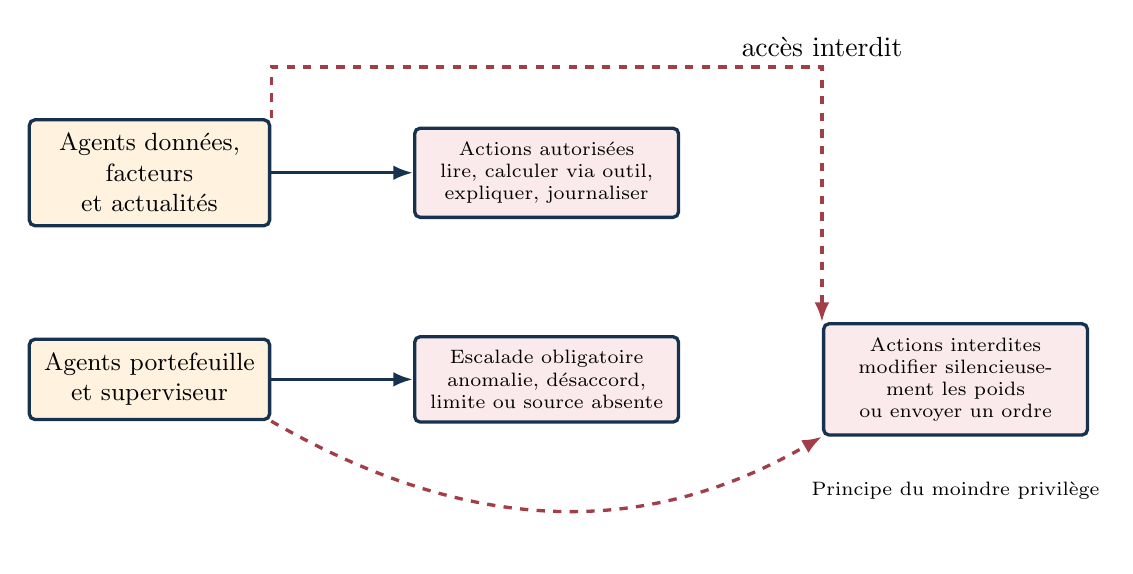
\begin{tikzpicture}[node distance=14mm and 9mm]
\node[agent, text width=2.7cm] (read)
  {Agents données, facteurs\\et actualités};
\node[agent, text width=2.7cm, below=of read] (recommend)
  {Agents portefeuille\\et superviseur};

\node[control, font=\scriptsize, text width=3.0cm, right=18mm of read] (allowed)
  {Actions autorisées\\lire, calculer via outil,\\expliquer, journaliser};
\node[control, font=\scriptsize, text width=3.0cm, right=18mm of recommend] (escalate)
  {Escalade obligatoire\\anomalie, désaccord,\\limite ou source absente};
\node[control, font=\scriptsize, text width=3.0cm, right=18mm of escalate] (forbidden)
  {Actions interdites\\modifier silencieusement les poids\\ou envoyer un ordre};

\draw[arrow] (read.east) -- (allowed.west);
\draw[arrow] (recommend.east) -- (escalate.west);

% Les accès interdits sont routés au-dessus et au-dessous des contrôles.
\draw[danger] (read.north east) -- ++(0,0.65cm)
  -| node[pos=0.5,above]{accès interdit} (forbidden.north west);
\draw[danger] (recommend.south east)
  to[out=-30,in=210] (forbidden.south west);

\node[label, below=5mm of forbidden] {Principe du moindre privilège};
\end{tikzpicture}
\end{document}\n